\section{Pilastro $P36$}
Il pilastro $P36$ è, in funzione dei piani, un pilastro d'angolo - cioè ha influenza solo verso l'interno dell'edificio, o di bordo - cioè divide i due ambienti interno ed esterno e quindi ha un'area di influenza anche sulla terrazza, o ancora un pilastro interno.

L'analisi di questo pilastro risulterà molto più laboriosa rispetto al precedente appunto per i motivi sopra descritti.

La sezione si articolerà il più possibile nella stessa maniera del precedente, dividendo in piani e studiandoli separatamente.

\subsection{Copertura}
In copertura il pilastro in esame risulta essere d'angolo. L'area di influenza è quella rappresentata in figura~\ref{fig:p36infAreaCopertura}.

\begin{figure}
	\centering
	\includegraphics[width=.6\textwidth]{p36_copertura}
	\caption{Area di influenza del pilastro $P36$ in copertura e al piano secondo}
	\label{fig:p36infAreaCopertura}
\end{figure}

Lato trave, lo schema statico è una trave a una campata semplicemente appoggiata. La distanza di influenza è quindi
\[
	l_1 = 0.5\cdot l = 0.5\cdot 4.00\,m = 2.00\,m
\]

Nell'altro senso, il solaio può essere schematizzato come a due campate; cioè
\[
	l_2 = \dfrac{3}{8}\,l = \dfrac{3}{8}\cdot 4.00\,m = 1.50\,m
\]

L'area di influenza è perciò pari a
\[
	A_{inf}^{cop} = 2.00\,m \cdot 1.50\,m = 3.00\,m^2
\]

Il carico strutturale del solaio genera la seguente azione sul pilastro
\begin{equation*}
		N_{G_1, solaio} = 3.60\,\dfrac{kN}{m^2} \cdot 3.00\,m^2 = 10.80\,kN
\end{equation*}

mentre il peso totale del pilastro è il medesimo del $P27$
\[
	N_{G_1, pilastro}^{tot} = 27.45\,kN
\]

Il peso strutturale delle travi, in funzione della lunghezza di influenza di quest'ultime ($2\,m$ per entrambe) è
\[
	N_{G_1, trave} = 3.75\,\dfrac{kN}{m}\cdot (2.00 + 2.00)\,m = 15\,kN
\]

I carichi non strutturali, tenendo conto che in copertura non sono presenti tamponamenti, sono
\[
		N_{G_2, solaio} = 2.84\,\dfrac{kN}{m^2}\cdot 3.00\,m^2 = 8.52\,kN
\]

Infine, i carichi variabili
\[
	\begin{cases}
		N_{Q_s} = 2.41\,\dfrac{kN}{m^2}\cdot 3.00\,m^2 = 7.23\,kN\\
		N_{Q_{CAT. H}} = 0.50\,\dfrac{kN}{m^2}\cdot 3.00\,m^2 = 1.50\,kN\\
		N_{Q_w} = \pm 0.138\,\dfrac{kN}{m^2}\cdot 3.00\,m^2 = \pm 0.414\,kN\\
	\end{cases}
\]
ricordando che in copertura è presente solo il carico da neve dovuto dal coefficiente di forma della copertura $\mu_1$ e che il vento può dare un effetto positivo o negativo a seconda della direzioni in cui spira.

\subsection{Piano Secondo}
Il secondo piano, come già detto, è fondamentalmente uguale alla copertura in termini di schema statico. Cambiano ovviamente i carichi, che sono
\[
	\begin{cases}
		N_{G_1, trave} = 3.75\,\dfrac{kN}{m}\cdot (2.00 + 2.00)\,m = 15\,kN\\\\
		N_{G_1, solaio} = 3.20\,\dfrac{kN}{m^2} \cdot 3.00\,m^2 = 9.60\,kN\\\\
		N_{G_2, solaio} = 4.62\,\dfrac{kN}{m^2} \cdot 3.00\,m^2 = 13.86\,kN\\\\
		N_{G_2, tamponamenti} = 10.48\,\dfrac{kN}{m} \cdot (2.00 + 2.00)\,m = 41.92\,kN\\\\
		N_{Q_{CAT.A}} = 2\,\dfrac{kN}{m^2} \cdot 3.00\,m^2 = 6.00\,kN
	\end{cases}
\]

\subsection{Piano Primo}
Il piano primo è forse quello più complicato di tutti riguardo il calcolo dell'area di influenza. Infatti, il pilastro è sul contorno che divide l'ambiente interno dalla terrazza esterna. L'area di influenza è sintetizzata in figura~\ref{fig:p36infAreaPianoPrimo}

\begin{figure}
	\centering
	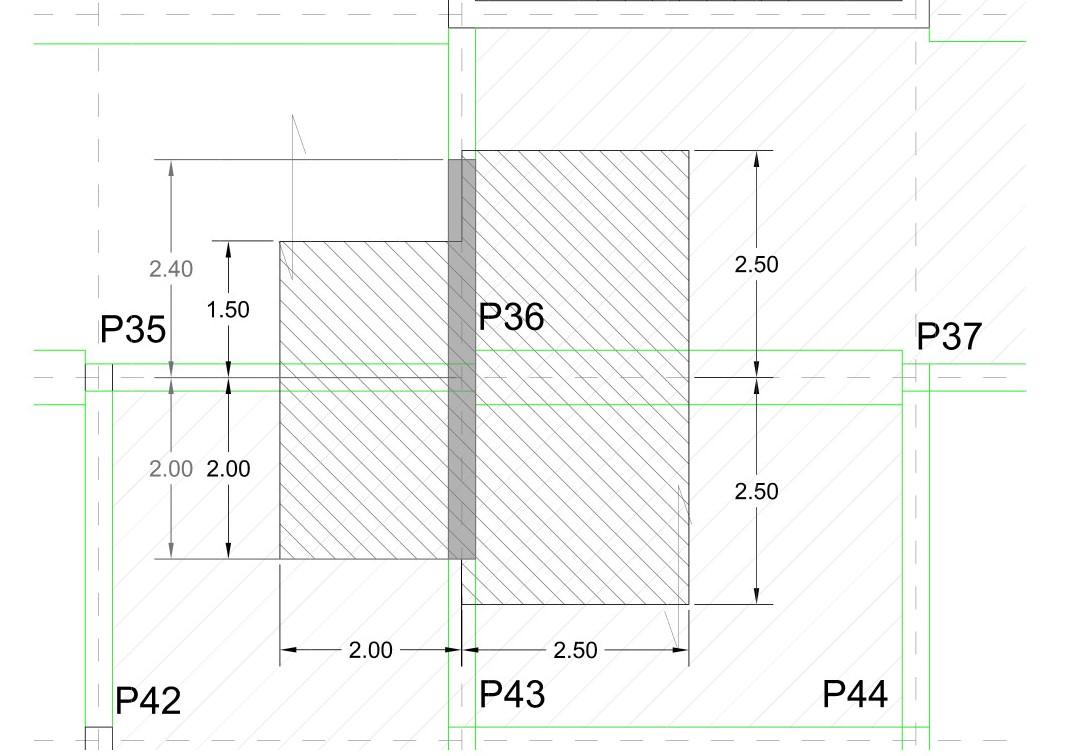
\includegraphics[width=.8\textwidth]{p36_pianoPrimo}
	\caption{Area di influenza del pilastro $P36$ al piano primo}
	\label{fig:p36infAreaPianoPrimo}
\end{figure}

L'area di influenza interna è di
\[
	A_{inf,int}^{P1} = 1.50\,m\cdot2.00\,m = 3.00\,m^2
\]
mentre quella esterna è di 
\[
	A_{inf, ext}^{P1} = (2.50+2.50)\,m \cdot 2.50\,m  + 2.00\,m \cdot 2.00\,m = 16.50\,m^2
\]

Il peso totale delle travi per il piano primo è di
\[
	N_{G_1, trave} = 3.75\,\dfrac{kN}{m}\cdot (2.00 + 2.50 + 2.40 + 2.00)\,m = 33.375\,kN
\]
mentre i tamponamenti
\[
	N_{G_2, tamponamenti} = 9.20\,\dfrac{kN}{m} \cdot (2.00 +2.40)\,m = 40.48\,kN
\]


Si ha ora la necessità di suddividere in parte interna e parte esterna.

\subsubsection*{Solaio interno}
Il solaio interno, genera le seguenti azioni sul pilastro in esame
\[
	\begin{cases}
		N_{G_1, solaio} = 3.20\,\dfrac{kN}{m^2} \cdot 3.00\,m^2 = 9.60\,kN\\\\
		N_{G_2, solaio} = 4.62\,\dfrac{kN}{m^2} \cdot 3.00\,m^2 = 13.86\,kN\\\\
		N_{G_2, tamponamenti} = 10.48\,\dfrac{kN}{m} \cdot (2.00 + 2.00)\,m = 41.92\,kN\\\\
		N_{Q_{CAT.B2}} = 3\,\dfrac{kN}{m^2} \cdot 3.00\,m^2 = 9.00\,kN
	\end{cases}
\]

\subsubsection*{Terrazza}
Lato terrazza, le azioni generate sono le seguenti
\[
	\begin{cases}
		N_{G_1, terr} = 3.20\,\dfrac{kN}{m^2} \cdot 16.50\,m^2 = 52.80\,kN\\\\
		N_{G_2, terr} = 2.215\,\dfrac{kN}{m^2} \cdot 16.50\,m^2 = 36.55\,kN\\\\
		N_{Q_{CAT.B}} = 4.00\,\dfrac{kN}{m^2} \cdot 16.50\,m^2 = 66.00\,kN\\\\
		N_{Q_{s}} = 4.90\,\dfrac{kN}{m^2} \cdot 16.50\,m^2 = 80.85\,kN\\\\
		N_{Q_{w}} = \pm0.138\frac{kN}{m^2} \cdot 16.50\,m^2 = \pm 2.28\,kN
	\end{cases}
\]

\subsection{Piano Terra}
Al piano terra il pilastro è interno. L'area di influenza è descritta dalla figura~\ref{fig:p36infAreaPianoTerra}.

\begin{figure}
	\centering
	\includegraphics[width=.8\textwidth]{p36_pianoTerra}
	\caption{Area di influenza del pilastro $P36$ al piano terra}
	\label{fig:p36infAreaPianoTerra}
\end{figure}

L'area di influeza al piano terra risulta essere
\[
	A_{inf}^{PT} = (1.00\cdot 2.00 + 3.00\cdot2.00 + 2.00\cdot 2.00)\,m^2 = 18\,m^2
\]

Le azioni generate dai carichi sono
\[
	\begin{cases}
		N_{G_1, solaio} = 3.60\,\dfrac{kN}{m^2} \cdot 18.00\,m^2 = 64.80\,kN\\\\
		N_{G_1, trave} = 3.75\,\dfrac{kN}{m}\cdot (2.00 + 3.00 + 2.00)\,m = 26.25\,kN\\\\
		N_{G_2, solaio} = 4.62\,\dfrac{kN}{m^2} \cdot 18.00\,m^2 = 83.16\,kN\\\\
		N_{Q_{CAT.D1}} = 4.00\,\dfrac{kN}{m^2} \cdot 18.00\,m^2 = 72.00\,kN
	\end{cases}
\]

Essendo un pilastro interno, non sono presenti tamponamenti che agiscono sulle travi.

\subsection{Combinazione agli SLU}
Dalla combinazione fondamentale si ricave che il massimo si ha massimizzando l'azione della neve.

\begin{align*}
	N_{max}^{P36} =& 1.3\cdot(27.45 + 15 +10.8 + 15+9.60 + 33.375+9.60+52.80+64.80+26.25)+\\
	&+1.5\cdot(8.52+13.86+41.92+13.86+36.55+40.48+83.16)+\\
	&+1.5\cdot(7.23+0\cdot1.5+0.6\cdot0.414+6+0.7\cdot9+0.7\cdot66+80.85+0.6\cdot2.28+72) =\\
	=& 1031.89\,kN
\end{align*}

Il diagramma dell'andamento delle azioni è riportato in figura~\ref{fig:P36axialLoad_slu}

\begin{figure}
	\centering
	\subfloat[\emph{Andamento dell'azione assiale massima sul pilastro $P36$}]{
	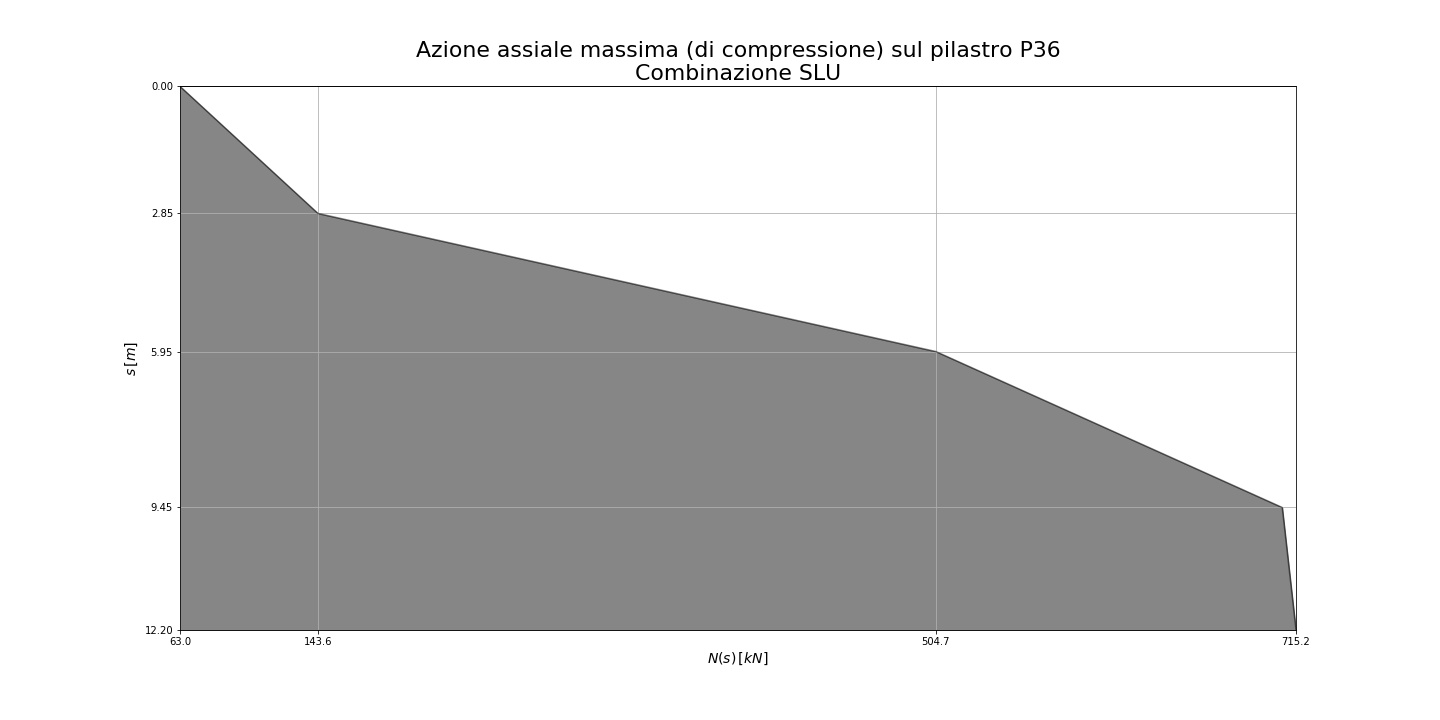
\includegraphics[width=.8\textwidth]{../../export/img/P36_maxAxialLoad_slu}}\\
	\subfloat[\emph{Andamento dell'azione assiale minima sul pilastro $P36$}]{
	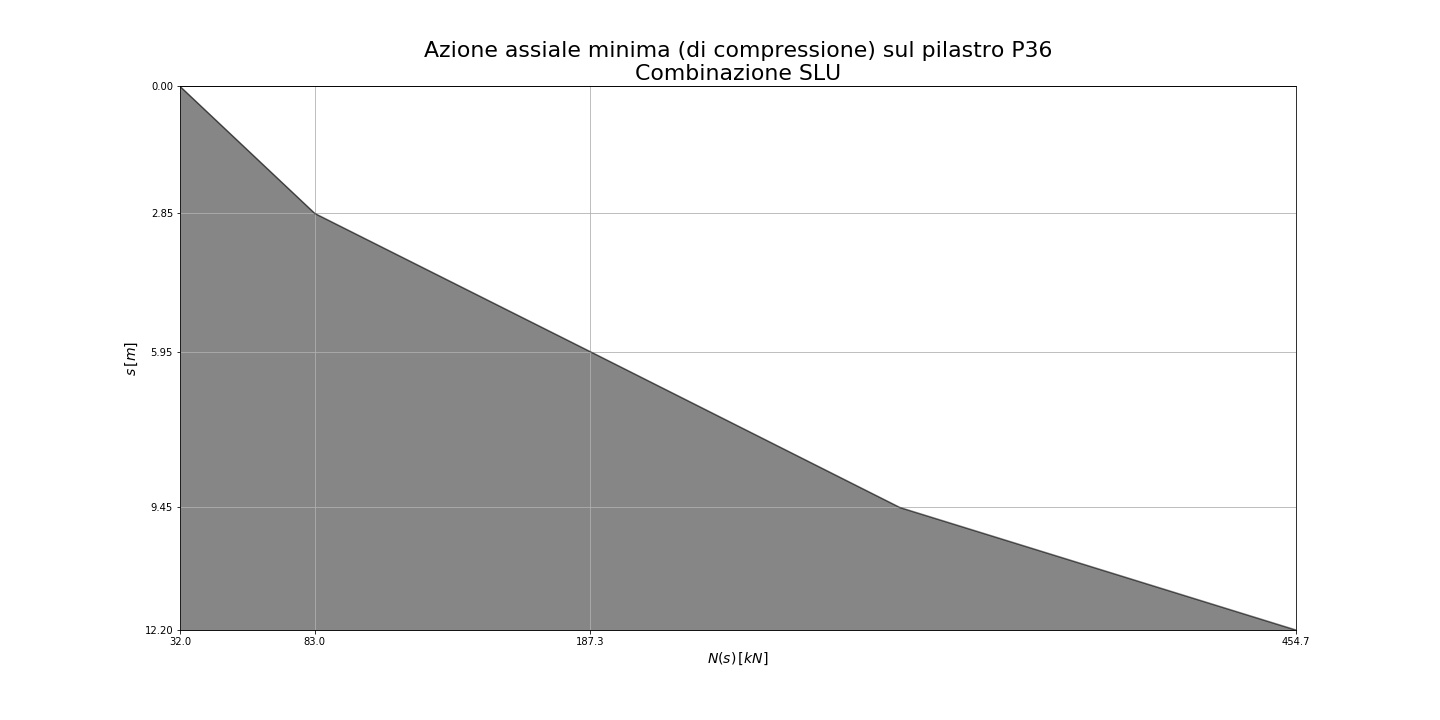
\includegraphics[width=.8\textwidth]{../../export/img/P36_minAxialLoad_slu}}
	\caption{Andamento delle azioni interne di compressione sul pilastro $P36$ in combinazione SLU}
	\label{fig:P36axialLoad_slu}
\end{figure}

\begin{align*}
	N_{min}^{P36} =& 1\cdot(27.45 + 15 +10.8 + 15+9.60 + 33.375+9.60+52.80+64.80+26.25)+\\
	&+0.8\cdot(8.52+13.86+41.92+13.86+36.55+40.48+83.16)+\\
	&+0 - 1.5\cdot(0.414 + 2.28) =\\
	=& 451.314\,kN
\end{align*}

\subsection{Combinazione agli SLE rara}

\begin{align*}
	N_{max}^{P36} =&(27.45 + 15 +10.8 + 15+9.60 + 33.375+9.60+52.80+64.80+26.25)+\\
	&+(8.52+13.86+41.92+13.86+36.55+40.48+83.16)+\\
	&(7.23+0\cdot1.5+0.6\cdot0.414+6+0.7\cdot9+0.7\cdot66+80.85+0.6\cdot2.28+72) =\\
	=& 717.82\,kN
\end{align*}

\begin{figure}
	\centering
	\subfloat[\emph{Andamento dell'azione assiale massima sul pilastro $P36$}]{
	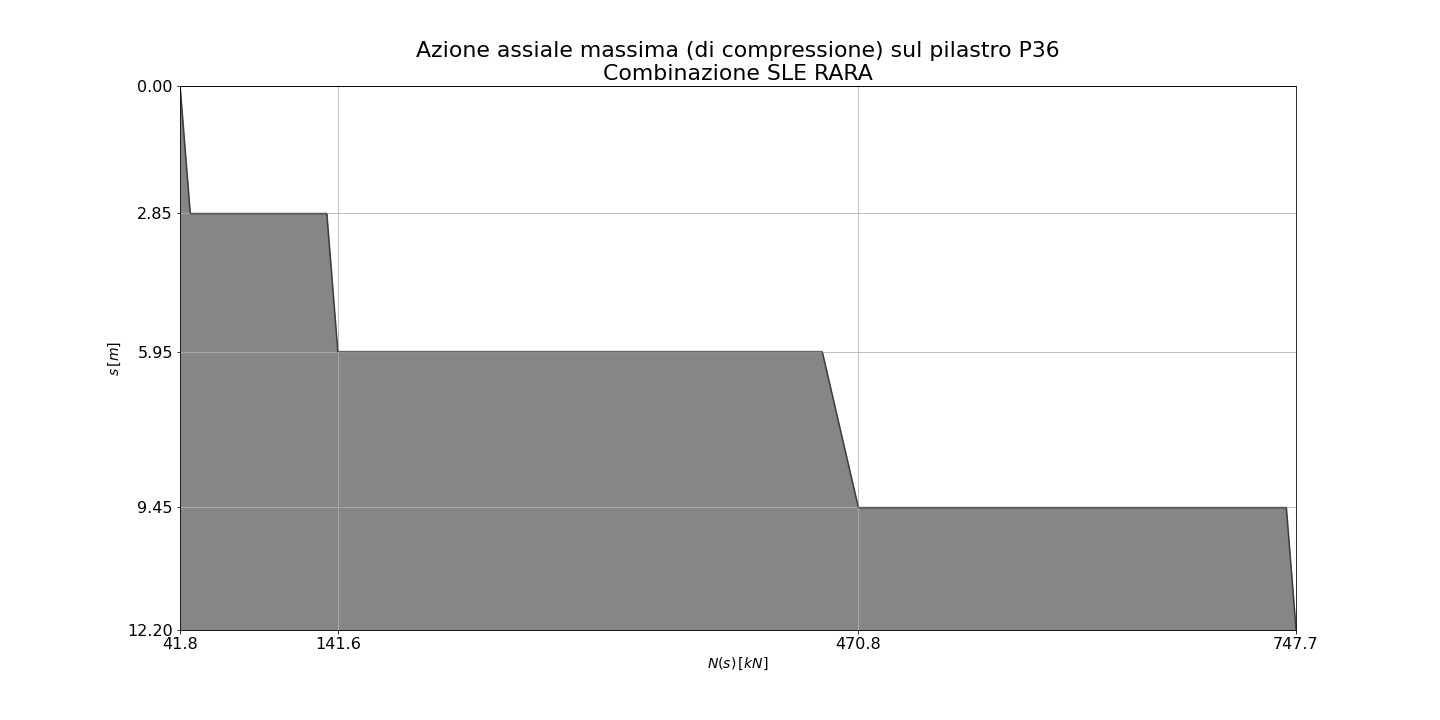
\includegraphics[width=.8\textwidth]{../../export/img/P36_maxAxialLoad_sleRara}}\\
	\subfloat[\emph{Andamento dell'azione assiale minima sul pilastro $P36$}]{
	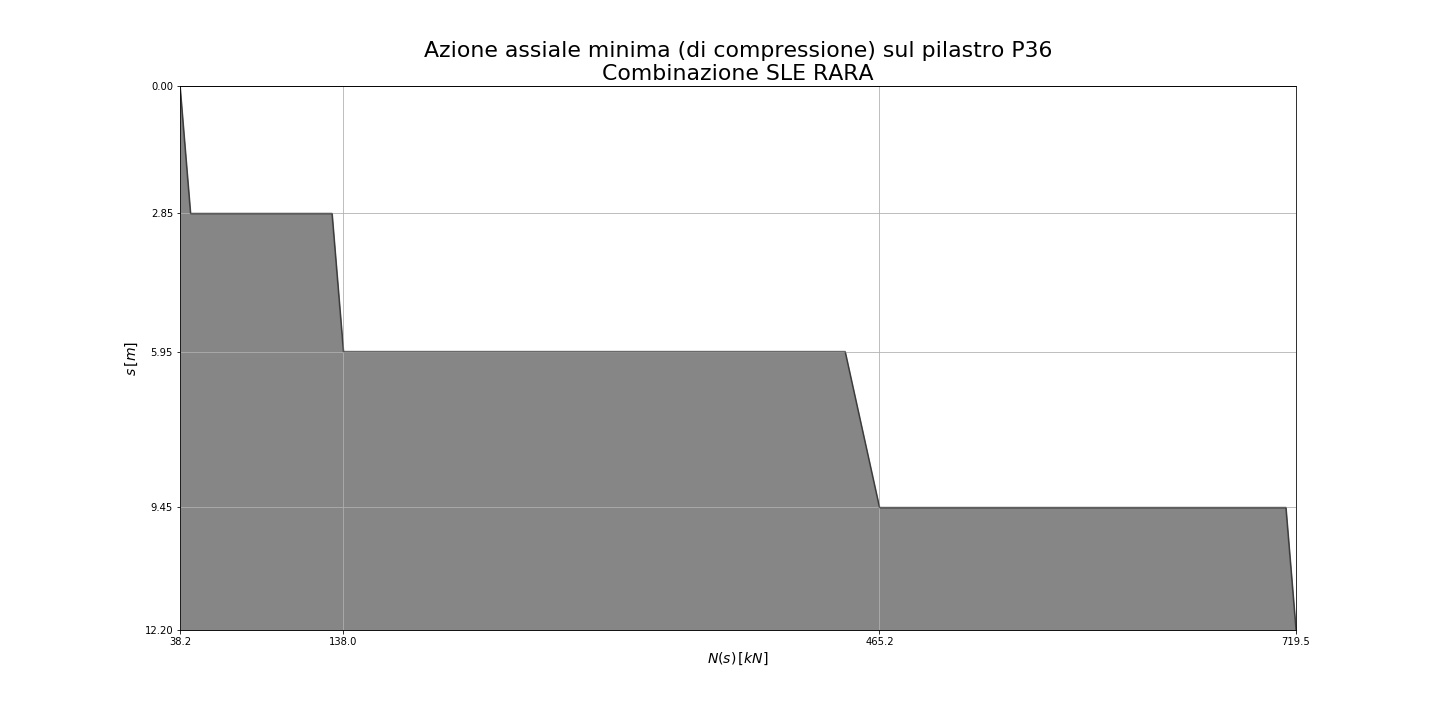
\includegraphics[width=.8\textwidth]{../../export/img/P36_minAxialLoad_sleRara}}
	\caption{Andamento delle azioni interne di compressione sul pilastro $P36$ in combinazione SLE rara}
	\label{fig:P36axialLoad_sleRara}
\end{figure}

\begin{align*}
	N_{min}^{P36} =& (27.45 + 15+10.8 + 15+9.60 + 33.375+9.60+52.80+64.8+26.25)+\\
	&+(8.52+13.86+41.92+13.86+36.55+40.48+83.16)+\\
	&+(0.5\cdot7.23+0\cdot1.5+0.414+6+0.7\cdot9+0.7\cdot66+0.5\cdot80.85+2.28+72)=\\
	=& 680.259\,kN
\end{align*}

Il massimo si ha massimizzando l'azione della neve mentre il minimo massimizzando il carico dovuto al vento.

\subsection{Combinazione agli SLE frequente}

\begin{align*}
	N_{max}^{P36} =&(27.45 + 15 +10.8 + 15+9.60 + 33.375+9.60+52.80+64.80+26.25)+\\
	&+(8.52+13.86+41.92+13.86+36.55+40.48+83.16)+\\
	&(0.2\cdot7.23+0\cdot1.5+0\cdot0.414+0.3\cdot6+0.3\cdot9\\
	&+0.3\cdot66+0.2\cdot80.85+0\cdot2.28+0.6\cdot72) =\\
	=& 588.141\,kN
\end{align*}

\begin{figure}
	\centering
	\subfloat[\emph{Andamento dell'azione assiale massima sul pilastro $P36$}]{
	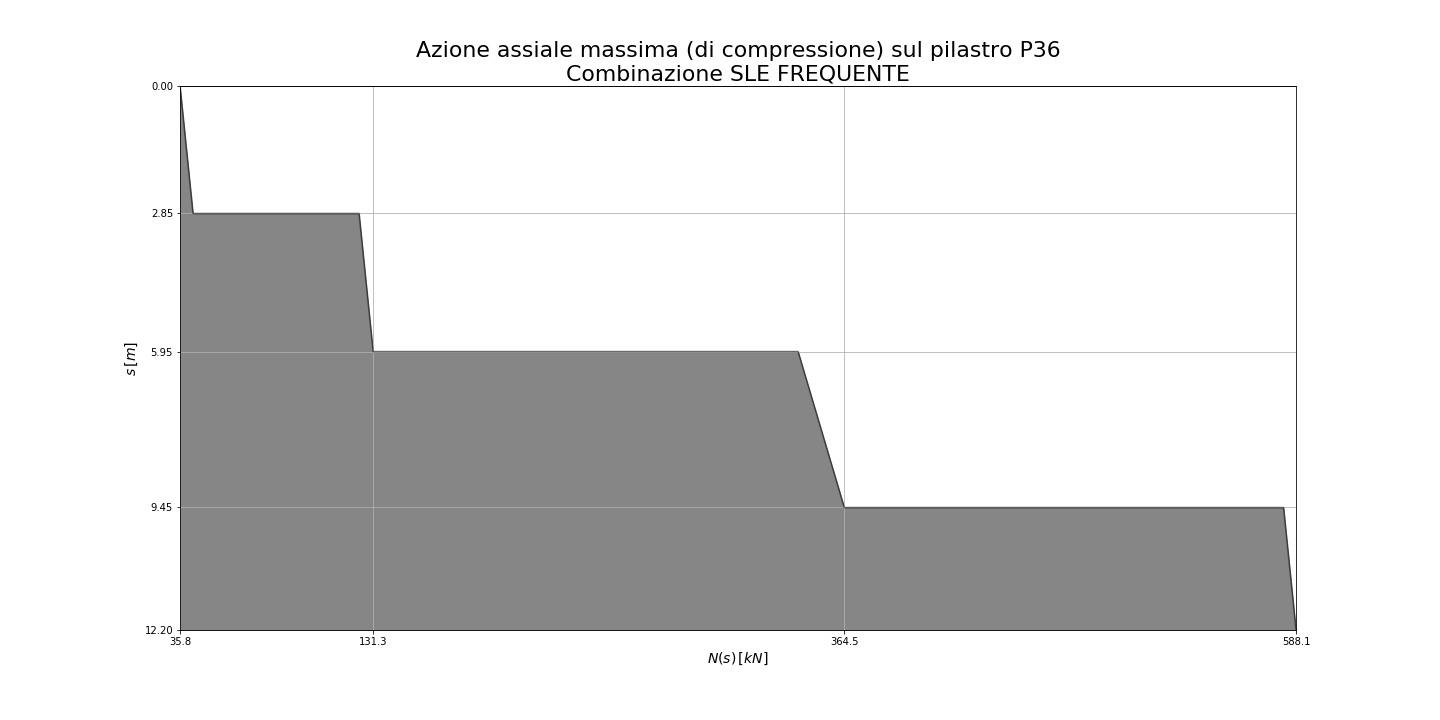
\includegraphics[width=.8\textwidth]{../../export/img/P36_maxAxialLoad_sleFreq}}\\
	\subfloat[\emph{Andamento dell'azione assiale minima sul pilastro $P36$}]{
	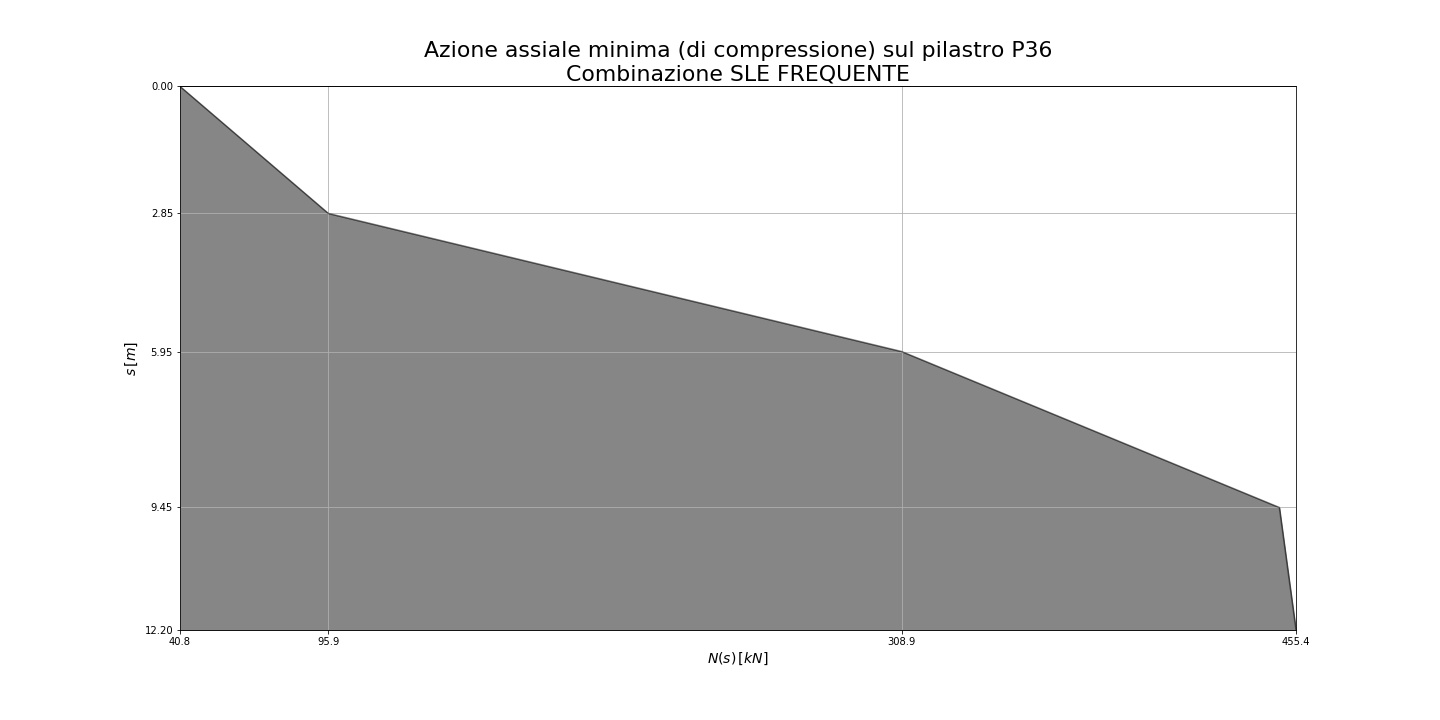
\includegraphics[width=.8\textwidth]{../../export/img/P36_minAxialLoad_sleFreq}}
	\caption{Andamento delle azioni interne di compressione sul pilastro $P36$ in combinazione SLE frequente}
	\label{fig:P36axialLoad_sleFreq}
\end{figure}

\begin{align*}
	N_{min}^{P36} =& (27.45 + 15+10.8 + 15+9.60 + 33.375+9.60+52.80+64.8+26.25)+\\
	&+(8.52+13.86+41.92+13.86+36.55+40.48+83.16)+\\
	&+(0\cdot7.23+0\cdot1.5+0.2\cdot0.414+0.3\cdot6+0.3\cdot9+\\
	&+0.3\cdot66+0\cdot80.85+0.2\cdot2.28+0.6\cdot72)=\\
	=& 572.06\,kN
\end{align*}

Anche in questo caso, il massimo si ha considerando il carico neve come principale, mentre il minimo considerando il vento.

\subsection{Combinazione agli SLE quasi permanente}

Per la combinazione quasi permanente si ha una sola combinazione

\begin{align*}
	N^{P36} =&(27.45 + 15 +10.8 + 15+9.60 + 33.375+9.60+52.80+64.80+26.25)+\\
	&+(8.52+13.86+41.92+13.86+36.55+40.48+83.16)+\\
	&+(0\cdot7.23+0\cdot1.5+0.2\cdot0.414+0.3\cdot6+0.3\cdot9+\\
	&+0.3\cdot66+0\cdot80.85+0.2\cdot2.28+0.6\cdot72) =\\
	=& 570.525\,kN
\end{align*}

\begin{figure}
	\centering
	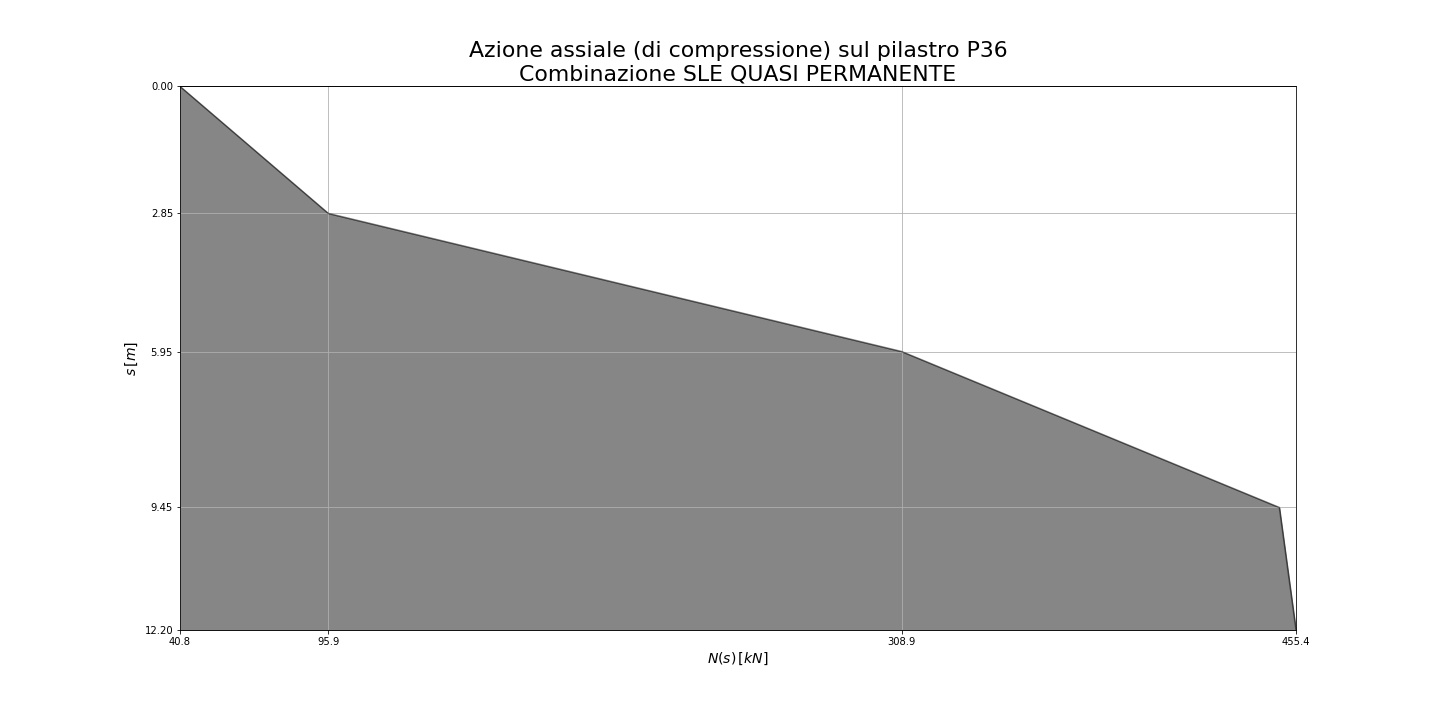
\includegraphics[width=.8\textwidth]{../../export/img/P36_axialLoad_sleQP}
	\caption{Andamento delle azioni interne di compressione sul pilastro $P36$ in combinazione SLE quasi permanente}
	\label{fig:P36axialLoad_sleQP}
\end{figure}

